%!TEX root = ../main.tex
\chapter{Commissioning of the AHCAL technological prototype}

Before every testbeam, all the electronics of the detector must be characterized. Before the full assembly, each individual chips must be tested in order to reject chips that presents bad channels or any other defects. After the assembly, each board needs to be characterized. This included the measurement of the SiPM-tile gain, the trigger threshold and electronic noise. In this chapter, the testing of the chips and the commissioning procedure of the AHCAL will be presented.

\section{Testing of individual SPIROC2B chips}

The testing of individual chips prior to the soldering to the HBU board is necessary. This avoids broken chips to be installed and reduces the number of dead channels. So far, the testing had to be done manually for each chip. This reduces the number of cross-checks done on the chips due to time constraints. The SPIROC2B chip can be tested standalone on a custom made PCB board. The SPIROC2B chip is installed in a special socket and is readout out by an ALTERA FPGA. The board is operated by a Labview software made by the OMEGA group \cite{OmegaWeb}.

\begin{figure}[htbp!]
  \centering
  \begin{subfigure}[t]{0.49\textwidth}
    \includegraphics[width=1.\linewidth]{chap4/fig_Commi/TestBoard.jpg}
    \caption{} \label{fig:Testboard_SP2B}
  \end{subfigure}
  \hfill
  \begin{subfigure}[t]{0.49\textwidth}
    \includegraphics[width=1.\linewidth]{chap4/fig_Commi/AnalogSignalSP2B.jpeg}
    \caption{} \label{fig:AnalogSignal_SP2B}
  \end{subfigure}
  \caption{\subref{fig:Testboard_SP2B}) Testboard used to test the SPIROC2B chip standalone. \subref{fig:AnalogSignal_SP2B}) Example of an analog signal outputted by the slow shaper of the SPIROC2B. The signal is represented in yellow. The trigger is represented in red.}
\end{figure}

The board as shown in figure \ref{fig:Testboard_SP2B} contains all the debugging feature needed to check the functioning of the chip. In red, the input signal pulse, generally similar to a SiPM pulse with a fast rising edge (around 1 ns) and a slower falling edge (around 20 ns), can be injected to the 36 channels of the chip. In blue and yellow are the output signals, this enables to check via an oscilloscope the output analog signal after the slow shaper as shown in figure \ref{fig:AnalogSignal_SP2B}, but can only be checked in external trigger mode. In purple, these are the input signals for the FPGA such as the slow clock, external trigger signals. And finally, in green, the DACs can be tested individually or automatically by connecting a Keithley multimeter to the serial port.

In this manual procedure, only vital parts of the chips are tested. This includes to check that all channels are working correctly, the chip works in both external and auto-trigger modes, all the DACs of the chip are working and that the digital part provides data. For the testbeam in July 2015, around 60 chips have been tested manually. The mean time for a chip to be tested was around 10 mins.

\subsection{DAC Testing}

As the testing procedure is done manually, only the most critical components of the chip needed to be tested. One of them is called the DAC which regulates the voltage channel-wise to the SiPM or the threshold discriminator. The procedure was done in two parts. First a simple check by checking the voltage on the channel at a value of 0. If one of the channels presented an unstable voltage, it indicates likely that the input DAC is broken thus the chip was discarded. If it passed, then the input DAC curve was simply measured by connecting a Keithley to the serial port and use the automatic measurement procedure from the Labview software. The time required was around 1-2 mins per chip. The output was a list containing the DAC value (from 0 to 255) and the associated voltage. The reconstructed figures are shown in \ref{fig:IDAC} for the input DAC and output DAC \ref{fig:OutDAC}.

\begin{figure}[htbp!]
  \centering
  \begin{subfigure}[t]{0.49\textwidth}
    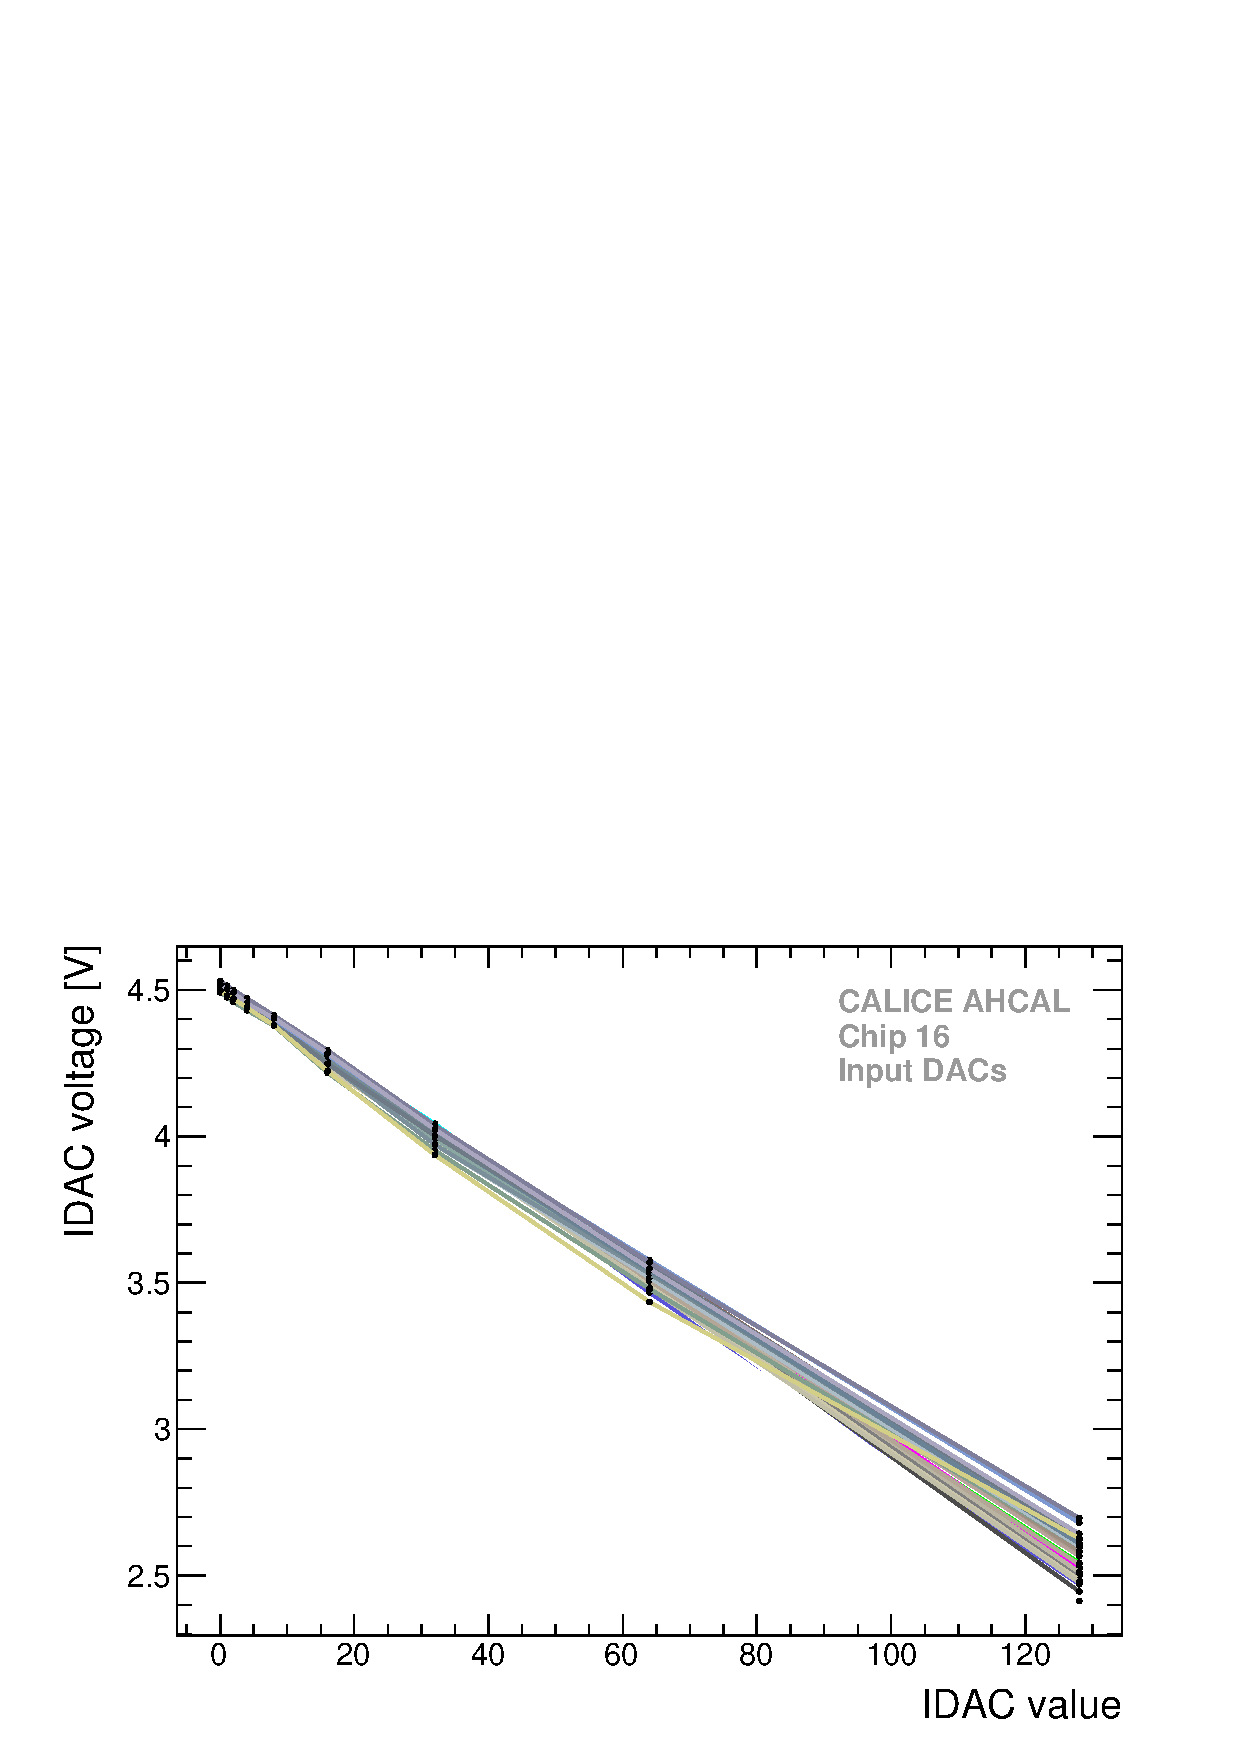
\includegraphics[width=1.\linewidth]{../Thesis_Plots/Commissioning/Plots/IDACs_Chip16.pdf}
    \caption{} \label{fig:IDAC}
  \end{subfigure}
  \hfill
  \begin{subfigure}[t]{0.49\textwidth}
    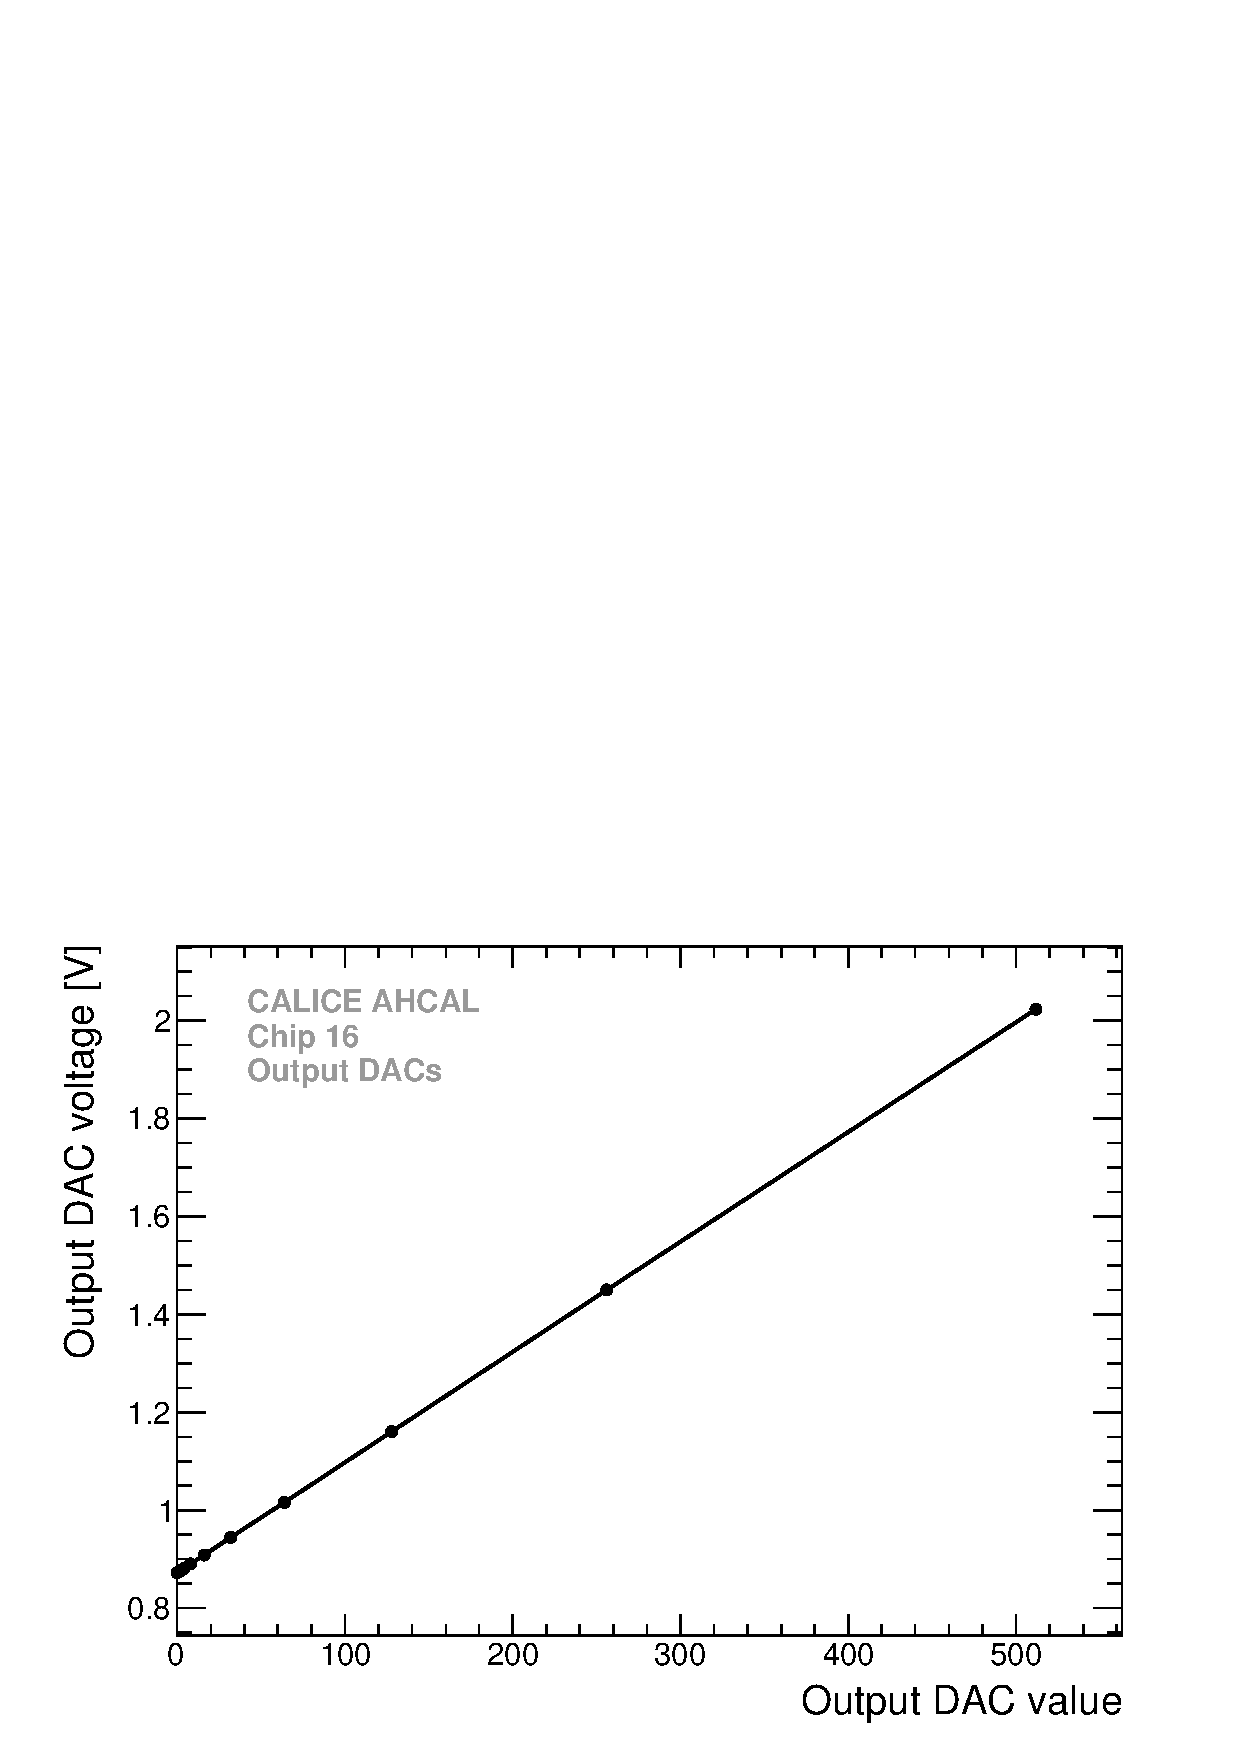
\includegraphics[width=1.\linewidth]{../Thesis_Plots/Commissioning/Plots/OutDACs_Chip16.pdf}
    \caption{} \label{fig:OutDAC}
  \end{subfigure}
  \caption{\subref{fig:IDAC}) Reconstructed input DAC curves of the 36 channels for the Chip 16 of the tested batch. \subref{fig:OutDAC}) Reconstructed output DAC curve for same tested chip.}
\end{figure}

One can notice that the spread channel-to-channel for the input DACs increases with the value. The spread is around 10 mV at a value of 0 and goes up to 200 mV at a value of 128. Thus for new produced boards, it has been chosen to use a value of 0 of the input DAC where the spread is minimal.

\begin{center}
  \rule{0.5\textwidth}{.4pt}
\end{center}

Around 60 chips were tested with a yield over 84\%. There is no obvious common cause for failure (digital part not working, no response to slow control programming, broken input DACs...). The time achieved by testing chips manually was around 10 mins which is not possible on a mass-production scale where only around 1 min is required at maximum per chip. This is why a new testing board has been designed between DESY and the University of Wuppertal in order to automatize the testing procedure of individual chips on BGA packaging \cite{AHCALMain2016_Amine}. This new board has already been commissioned in July 2017 and is being used currently for the next generation AHCAL prototype (around 650 chips).

\section{Commissioning procedure}

The commissioning procedure of the detector was done in July/August 2014 for a testbeam that was planned in October/November 2014 at the CERN PS facility. Mainly the same boards were used during the testbeams in 2015. Before the assembly of the detector into the absorber stack, each individual boards need to be tested. This test is done in order to characterize the full board assembled. The procedure is explained in details in \cite{Hartbrich2012} and was mainly done by these steps:

\begin{itemize}
  \item Setup the Power Board voltage to deliver to the SIPM and the input DAC value
  \item First characterization by measuring the SiPM gain at nominal settings
  \item Iterative adjustment of pre-amplifier to reach targeted SiPM gain
  \item Threshold scan measurement
  \item Noise measurement
\end{itemize}

The following subsections will describe each point into details. Only the new boards were fully commissioned. Old boards that were already calibrated used the same settings and only a cross-check was performed.

\subsection{Setting the High Voltage}

\begin{table}[htb!]
  \centering
  \caption{List of the different SiPMs used in the CALICE AHCAL in July 2015.}
  \label{table:sipm_list}
  \resizebox{\textwidth}{!}{%
  \begin{tabular}{cccccccc}
    \hline
    Layer & Producer & Model & Area (mm$^2$) & Pitch ($\mu$m) & WLS Fibre & Read-out type & $N_{px}$ [$10^3$]\\
    \hline
    1 & Hamamatsu & S12571\_010P & $1\times1$ & 10 & no & Bottom & 10\\
    2 & Hamamatsu & S10362-11-025O & $1\times1$ & 25 & no & Side & 1.6\\
    3 & Hamamatsu & S12571-025P & $1\times1$ & 25 & no & SMD & 1.6\\
    4-5 & Ketek & N/A & $2.25\times2.25$ & 18 & no & Side & 12\\
    6-10 & CPTA & CPTA & $1.28\times1.28$ & 40 & yes & Side & 0.8\\
    11-12 & Ketek & PM1125NS-SB0 & $1.2\times1.2$ & 25 & no & Side & 2.3\\
    13-14 & SenSL & MicroFB-10020-SMT & $1\times1$ & 20 & no & Side & 1.3\\
    \hline
  \end{tabular}
  }
\end{table}

An AHCAL board or HBU has 144 channels, each equipped with a plastic tile-SiPM. To achieve a certain light yield, meaning the number of fired pixels per MIP, the SiPM must be operated above a specific voltage called the breakdown voltage ($V_{Br}$). This voltage has been measured for a couple of SiPMs but it is generally given by the manufacturer where batches of SiPMs are placed in bags with a certain $V_{Br}$ and the lower/upper limits are indicated. The table \ref{table:sipm_list} shows the SiPMs used during the testbeam at CERN in July 2015. The variation of the breakdown voltage is in the order of hundreds of millivolts. As the quality of the SiPM has increased drastically in the last few years, the need for individual channel-wise voltage is reduced. Thus the chosen input DAC value was chosen to be 0 equivalent to -4.5V on the SiPM voltage pin. The SiPMs are operated between 2.5 to 5V over the breakdown voltage but varies with the type. The needed voltage to be applied and thus delivered by the power board is given by $V_{PB} [V] = V_{Br} + V_{overvoltage} + 4.5V$. The table \ref{table:Voltage_SiPM} sums up the voltages applied.

\begin{table}[htb!]
  \centering
  \caption{List of breakdown and operating voltages applied to each SiPM types. $V_{op}$ represents $V_{Br} + V_{overvoltage}$.}
  \label{table:Voltage_SiPM}
  \resizebox{\textwidth}{!}{%
  \begin{tabular}{@{} lccc @{}}
    \hline
    SiPM type \# & $V_{Br}$ & $V_{op}$ & $V_{PB}$\\
    \hline
    Hamamatsu (S12571\_010P - S10362-11-025O) & $\sim$ 65 V & $\sim$ 70 V & $\sim$ 75.8 V\\
    Hamamatsu (S12571-025P) & $\sim$ 65 V & $\sim$ 67 V & $\sim$ 70.66 V\\
    CPTA & $\sim$ 35-45 V & $\sim$ 37-50 V & $\sim$ 40.1 - 51.7 V\\
    Ketek & $\sim$ 28 V & $\sim$ 32 V & $\sim$ 36.95 - 37.02 V\\
    UHH Ketek & $\sim$ 27 V & $\sim$ 29.55 - 30.05 V & $\sim$ 32.98 - 34.49 V\\
    SenSL & $\sim$ 26 V & $\sim$ 27.391 - 27.392 V & $\sim$ 32.10 - 32.11 V\\
    \hline
  \end{tabular}
  }
\end{table}

\subsection{First characterization of the gain}

In this section, the SiPM gain is related to the ADC value between the two first peaks of a single pixel spectra where individual pixels, in a relatively small number (~10-15 pixels), are fired by an integrated LED system. This value is proportional to the high voltage applied to the SiPM and can be also modified by adjusting a feedback capacitor to the SPIROC2B high gain pre-amplifier. Before starting the gain measurement procedure, a holdscan needs to be performed. This procedure determines the necessary Hold time bits to set in the slow control configuration to sample the maximum of the signal. The procedure is simple, a fixed amplitude signal is injected via the LED integrated system to all the channels while repeating this for several Hold time values. The analysis enables to reconstruct the signal shape after the slow shaper and thus determine the Hold time necessary per chip as shown in figure \ref{fig:Holdscan}.

\begin{figure}[htbp!]
  \centering
  \begin{subfigure}[t]{0.49\textwidth}
    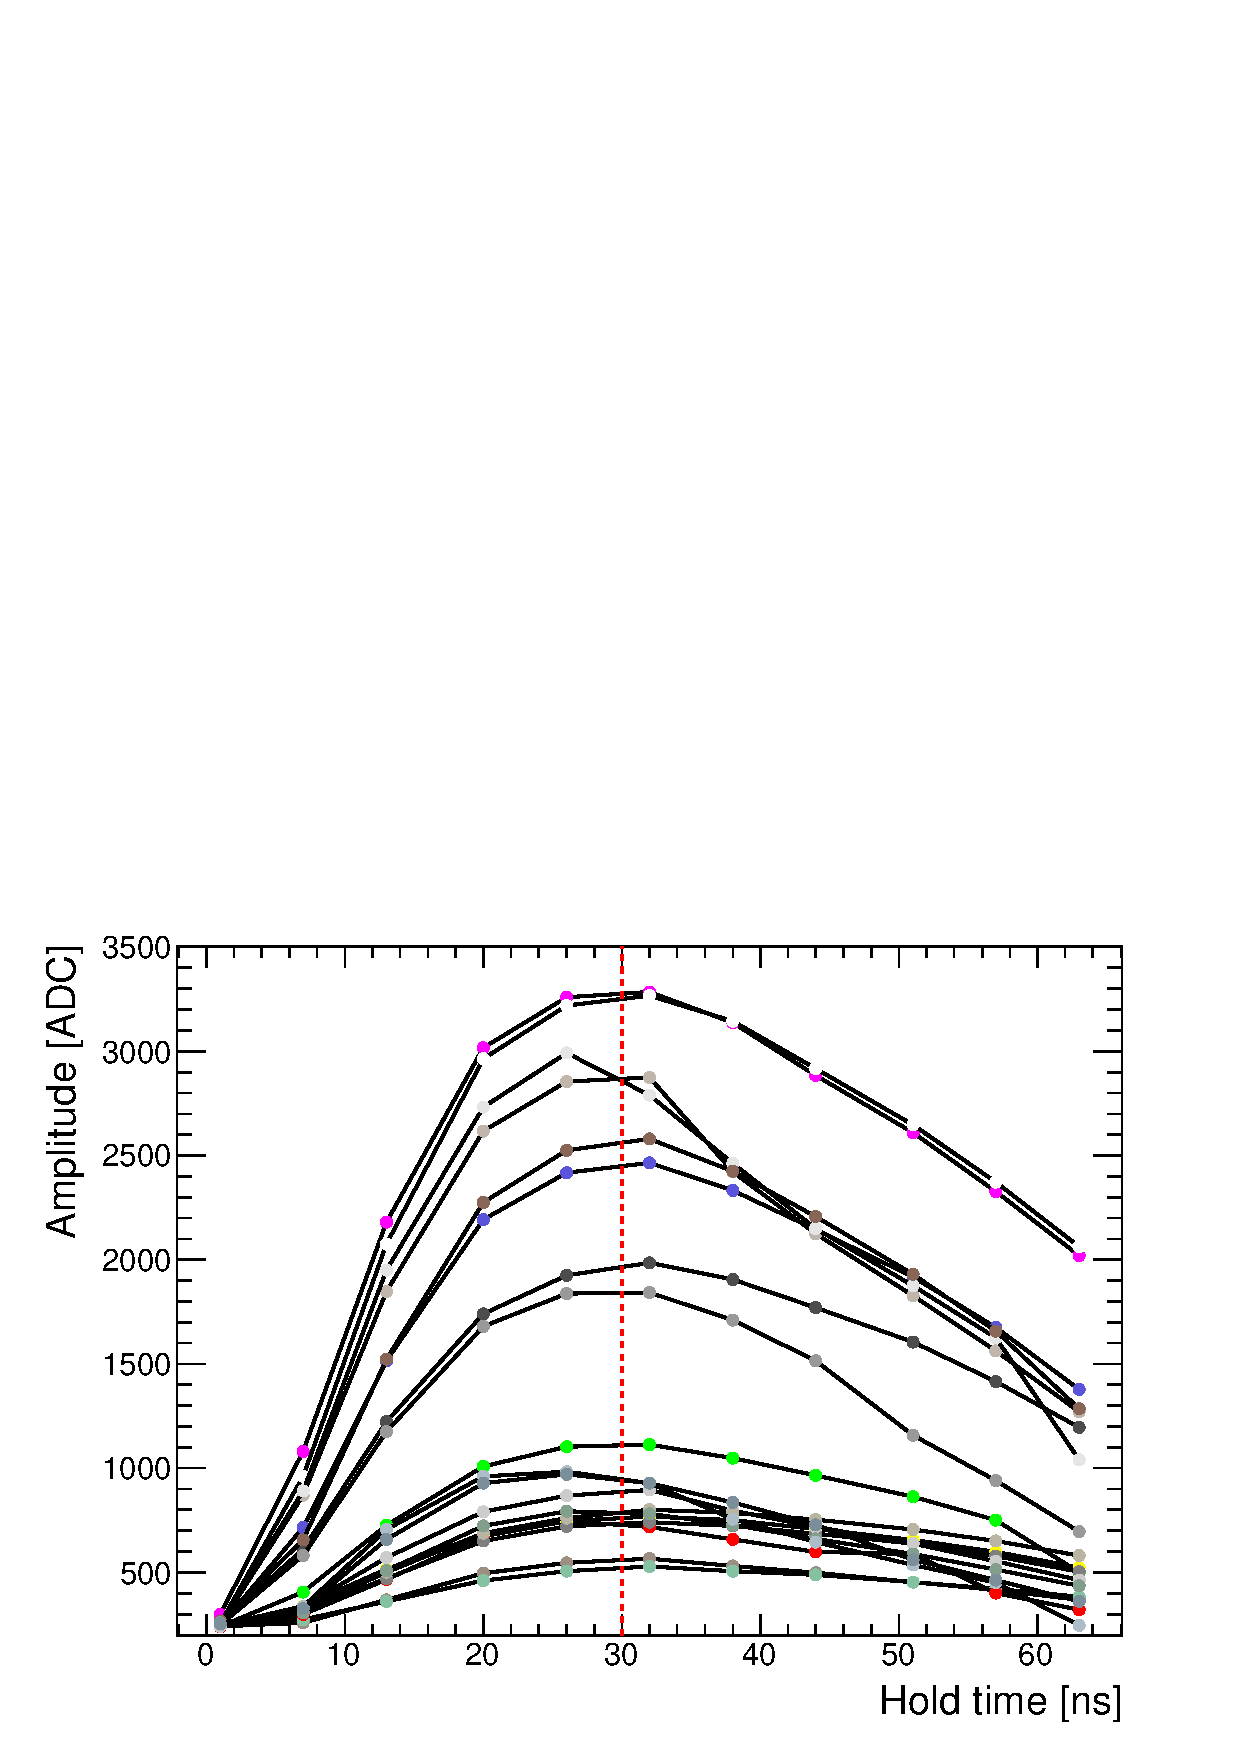
\includegraphics[width=1.\linewidth]{../Thesis_Plots/Commissioning/Plots/Holdscan_HBU2_15.pdf}
    \caption{Holdscan} \label{fig:Holdscan}
  \end{subfigure}
  \hfill
  \begin{subfigure}[t]{0.49\textwidth}
    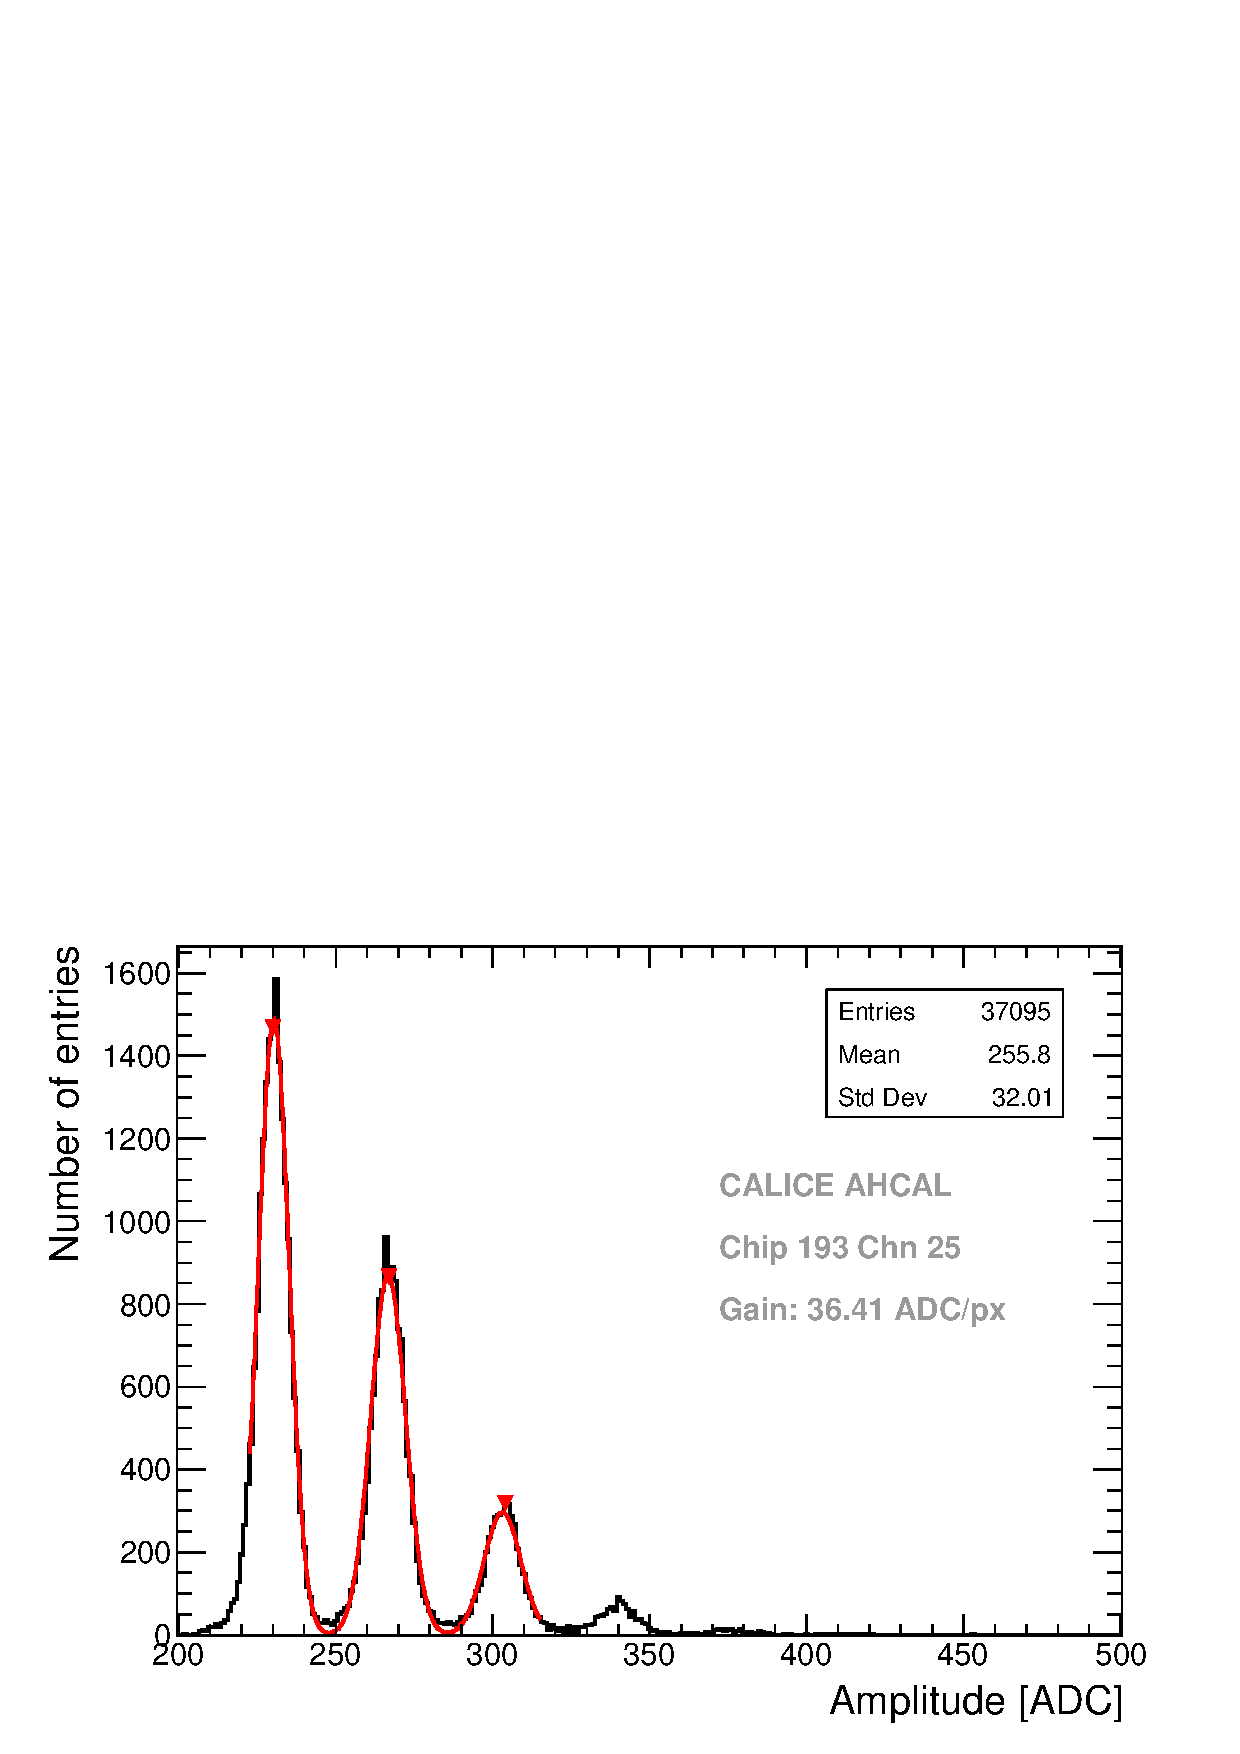
\includegraphics[width=1.\linewidth]{../Thesis_Plots/Commissioning/Plots/Gain100fF_MainzHBU4.pdf}
    \caption{Gain measured at 100 fF} \label{fig:Gain100fF}
  \end{subfigure}
  \caption{\subref{fig:Holdscan}) Reconstructed signal shape for several channels. The dotted red line represent the Hold time chosen for this board. \subref{fig:Gain100fF}) Single pixel spectra of a single channel. The fit is done by a Multi-Gaussian where the distance between the 1$^{st}$ and 2$^{nd}$ peaks is the fitted SiPM gain.}
\end{figure}

After this, a first characterization of the gain can be done at nominal settings using a pre-amplifier value of 100 fF. For this, all channels are illuminated by the LED system over a certain range of LED voltage by steps of 100 mV in order to characterize all channels (variation in response due to LED light, tiles, SiPM). In the case of old boards, a range of 10-15 voltages are generally needed but due to improvements for the new boards on the LED integrated calibration system, SiPM quality, tile quality, a much smaller range is used. The minimum used was 3 LED voltages to characterize all the channels. An example of a single pixel spectra at 100 fF can be seen in figure \ref{fig:Gain100fF}.

\subsection{Adjustment of the ADC dynamic range}

The goal of this procedure is to fit the dynamic range of the SPIROC2B in ADC to the number of pixels on the SiPM to avoid any ADC saturation before SiPM saturation. This calculation gives a good order of magnitude but is still approximative due to several unknown variables such as the number of effective pixels of a SiPM or the high/low gain intercalibration factor for each channel. The targeted gain is calculated by:

\begin{equation}
  G_{target} [ADC] = \frac{ADC_{max} \times IC [ADC]}{N_{px} [px]}
\end{equation}

where $G_{target}$ is the value targeted for gain, $ADC_{max}$ is the maximum ADC range, $IC$ the intercalibration and $N_{px}$ the number of pixels on the SiPM. The maximum ADC range factored with the intercalibration gives an approximated range of 36000 ADC (very conservative number) to avoid any saturation of the ADC. The table \ref{table:GainTarget_SiPM} sums up the calculated gains for each board. The new ITEP are operated in different modes for calibration and physics data due to the high number of pixels. The calibration mode is the operation at nominal settings (100 fF) and the physics mode is operated at the maximum pre-amplifier feedback capacitor value of 1500fF. The gain factor between both modes is around 7.

\begin{table}[htb!]
  \centering
  \caption{List of targeted gains for each layer.}
  \label{table:GainTarget_SiPM}
  \begin{tabular}{@{} cc @{}}
    \hline
    Type \# & $G_{target}$ [ADC] \\
    \hline
    Hamamatsu (S12571-025P) & $\sim$ 11\\
    CPTA & $\sim$ 22\\
    Ketek & $\sim$ 40 (calib) - 6 (physics)\\
    UHH Ketek & $\sim$ 16\\
    SenSL & $\sim$ 24\\
    \hline
  \end{tabular}
\end{table}

The pre-amplifier feedback capacitor value can be calculated using the figure \ref{fig:PA_curve}. In principle, this curve needs to be made for each channel but due to many improvements this curve gives a very good approximation. Using this curve, one can calculate the needed value for the feedback capacitor (rounded to the lower value) for a specifically targeted gain. In the example that is shown in figure \ref{fig:Gain100fF}, the calculation gives a value of 675 fF that need to be used to reach a gain of 12 ADC/px. The result of the fit is visible in figure \ref{fig:Gain675fF}. This procedure is iterated until the targeted gain is reached. %The gain fit results for this commissioning phase in August 2014 is available in appendix \ref{appendix:GainDistribuCommi}.

\begin{figure}[htbp!]
  \centering
  \begin{subfigure}[t]{0.49\textwidth}
    \includegraphics[width=1.\linewidth]{../Thesis_Plots/Commissioning/Plots/GainvsPA.pdf}
    \caption{} \label{fig:PA_curve}
  \end{subfigure}
  \hfill
  \begin{subfigure}[t]{0.49\textwidth}
    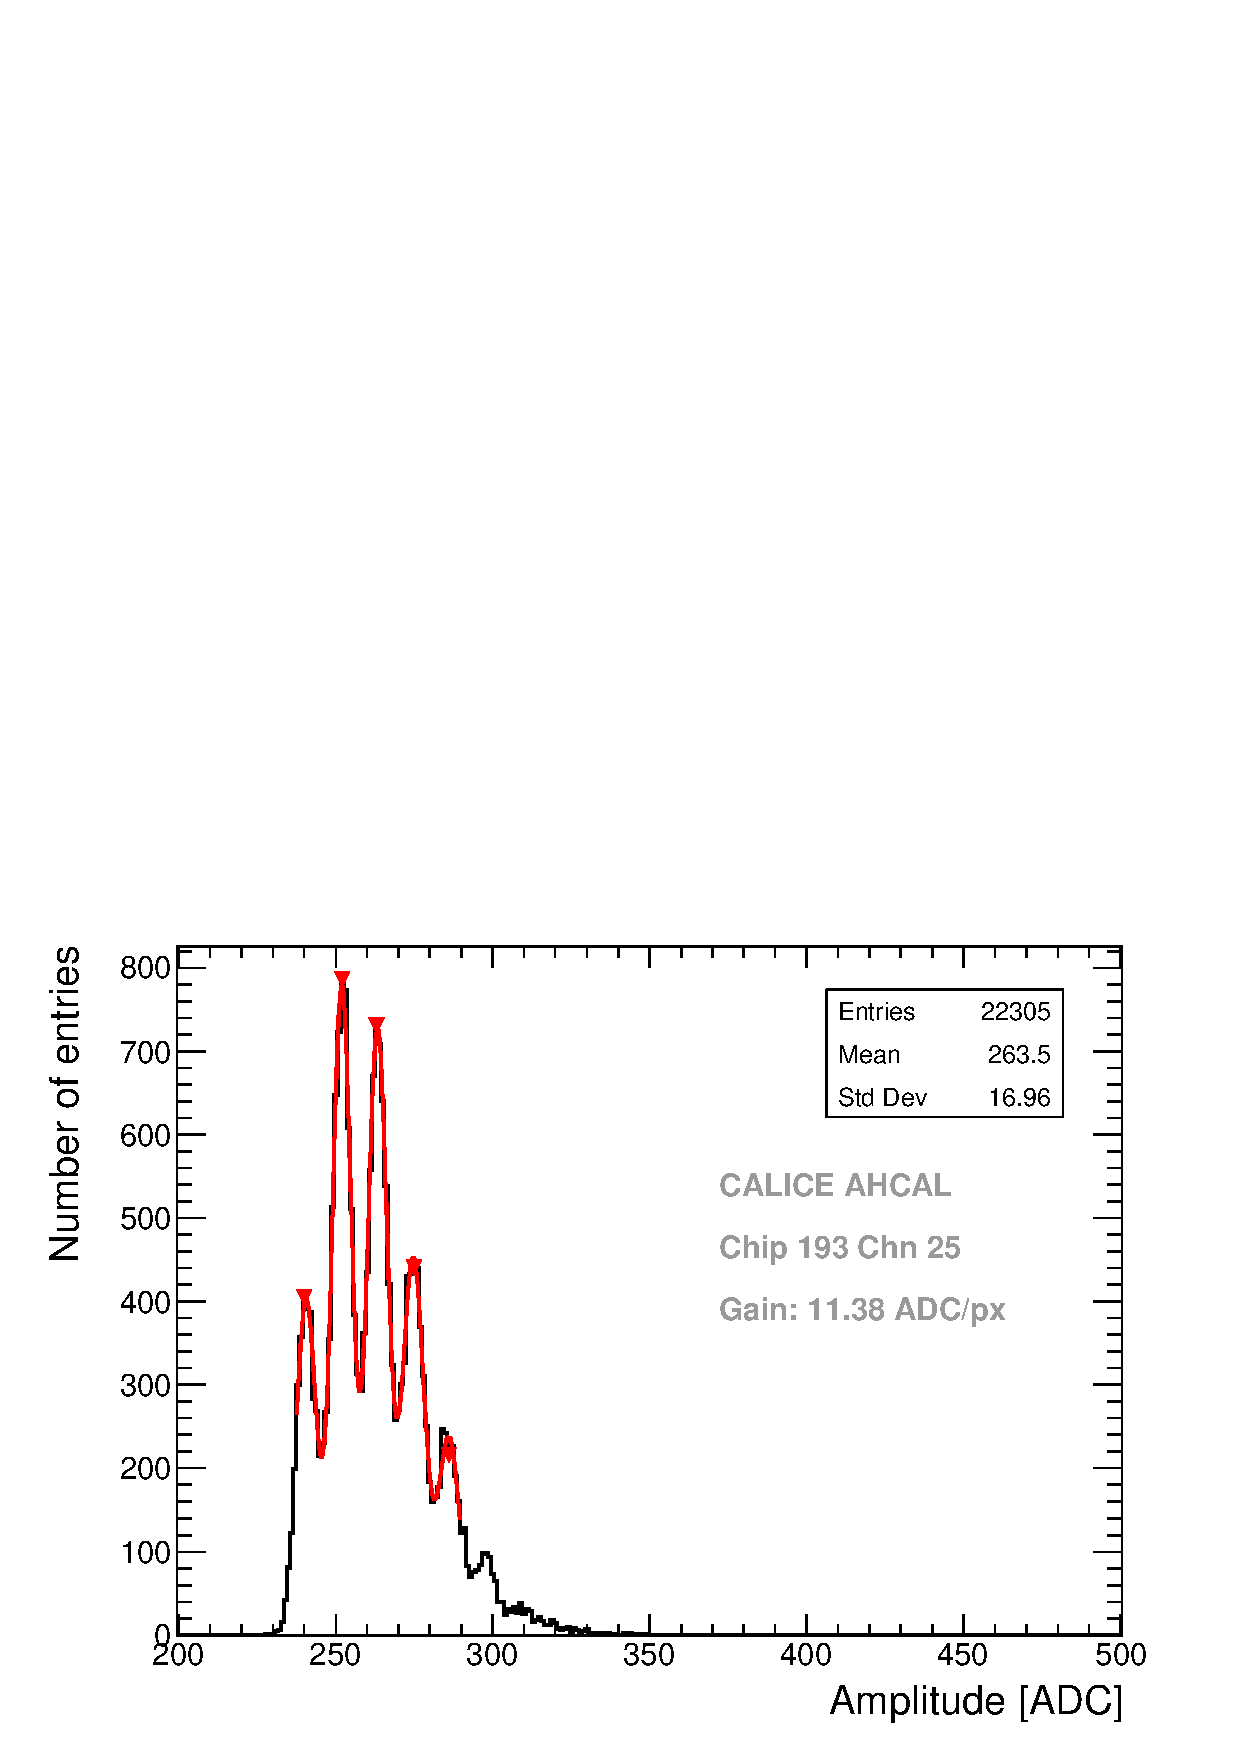
\includegraphics[width=1.\linewidth]{../Thesis_Plots/Commissioning/Plots/Gain675fF_MainzHBU4.pdf}
    \caption{} \label{fig:Gain675fF}
  \end{subfigure}
  \caption{\subref{fig:PA_curve}) Generic curve obtained with the new ITEP board used to determine the value of the pre-amplifier feedback capacitor to use. \subref{fig:Gain675fF}) Results of the gain fit for the same channel as shown above after adjustment of the pre-amplifier feedback capacitor from 100 fF to 675 fF.}
\end{figure}

\subsection{Threshold scan}

This procedure is rather new and was developed by a summer student in 2014. A better description of the procedure can been read in \cite{Hartbrich:2016bbz} and \cite{LloydTrigger}. The SPIROC2B offers the possibility of setting a global trigger threshold (10-bit range) as well as an individual channel-wise threshold (4-bit range) in auto-trigger operation. The trigger threshold needs to be setup properly in order to avoid loss of information if set too high or being overwhelmed by noise events if set too low. The goal of this method is to get a good idea (to an order of 5-10\%) of the needed value for the trigger threshold in a quick and efficient way.

\begin{figure}[htbp!]
  \centering
  \begin{subfigure}[t]{0.49\textwidth}
    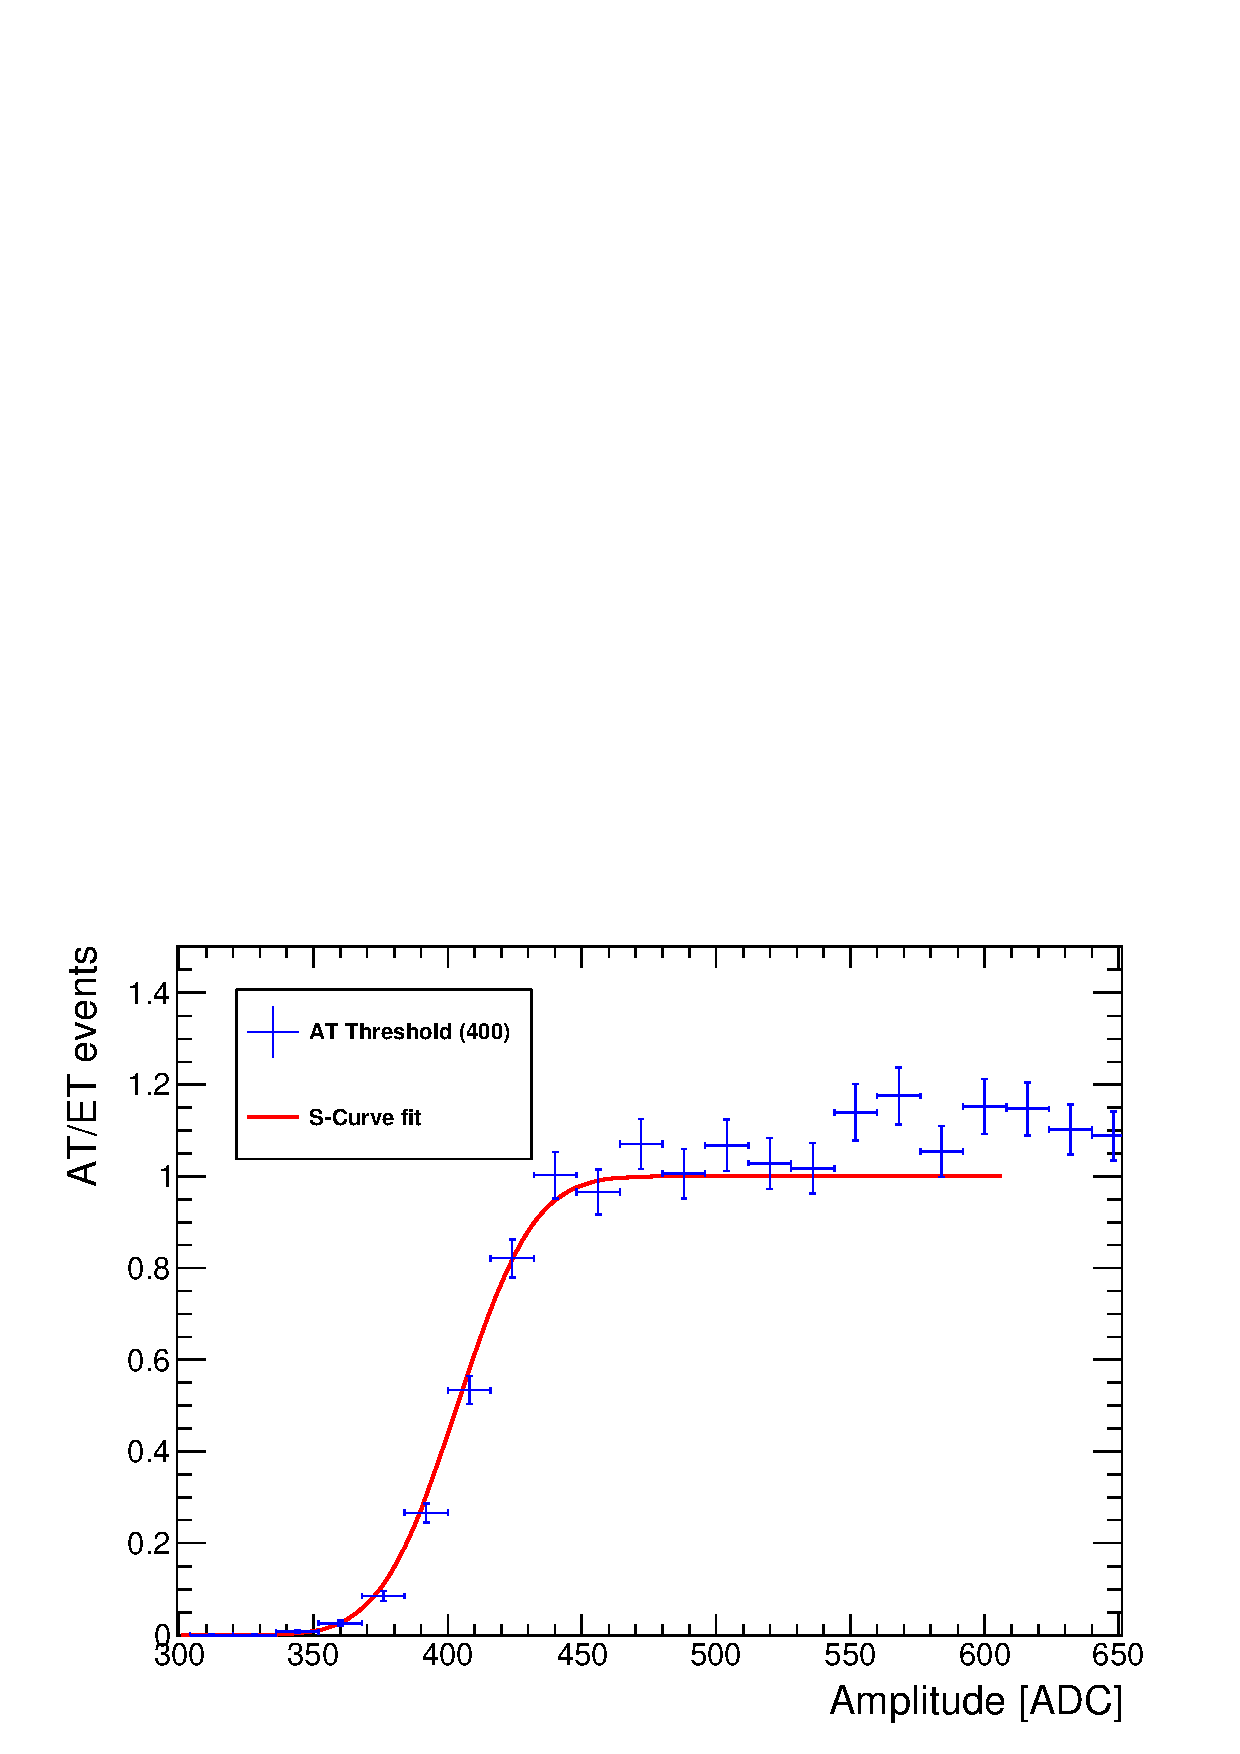
\includegraphics[width=1.\linewidth]{../Thesis_Plots/Commissioning/Plots/EfficiencyCurveFit_HBU2_12.pdf}
    \caption{} \label{fig:EffiCurve}
  \end{subfigure}
  \hfill
  \begin{subfigure}[t]{0.49\textwidth}
    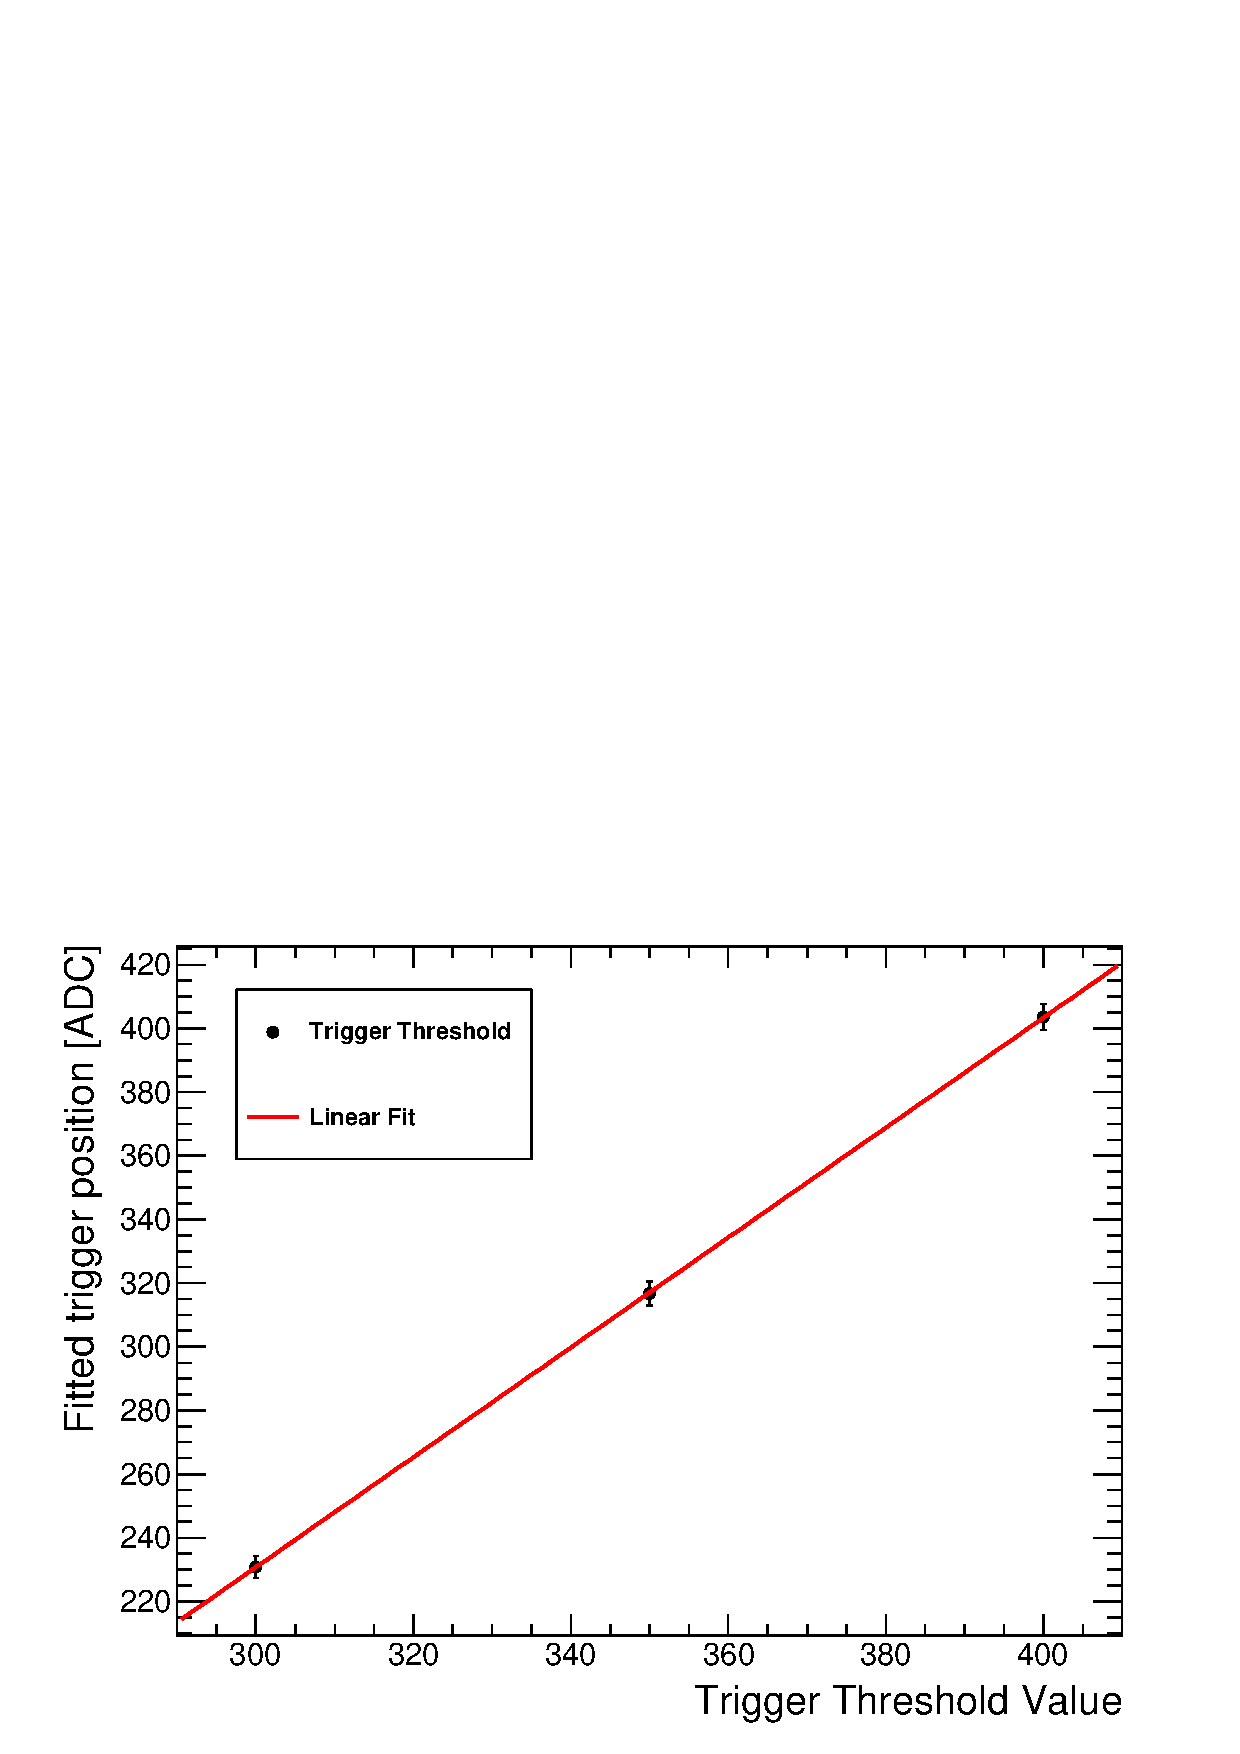
\includegraphics[width=1.\linewidth]{../Thesis_Plots/Commissioning/Plots/TriggerThresholdFit_HBU2_12.pdf}
    \caption{} \label{fig:TriggerFit}
  \end{subfigure}
  \caption{\subref{fig:EffiCurve}) Trigger efficiency S-Curve fit for a typical channel at a trigger threshold of 400. $\mu$ = 403.542 $\pm$ 4.04538. \subref{fig:TriggerFit}) Extracted trigger threshold positions as a function of the trigger threshold value. One can observe a linear behavior.}
\end{figure}

An example of the results for a single channel is shown in figure \ref{fig:EffiCurve} and \ref{fig:TriggerFit}. The efficiency is normalized to 1 due to the measurement method. The statistical uncertainty on the trigger position is around 1\% which is well below the needed accuracy. The dependence of the trigger position on the threshold parameter is linear as expected.

\section{Noise Measurement in the AHCAL}

Noise measurement is needed and complementary to the previous method. As explained above, the setting of the trigger threshold is very crucial. If the threshold is set too low, a noisy channel could overflow the whole detector thus reducing the readout efficiency. This method is a proof-of-concept that seems to fulfill the requirement of characterizing the threshold position for all the channels or a chip at once. The needed accuracy is also here not so crucial in order to keep the threshold in the acceptable range of 0.5 MIP. This method enables us to have an idea of the noise level at a certain trigger threshold and especially to understand the evolution of noise as a function of the trigger threshold. This measurement method utilizes the fact that SiPM noise should follow a Poisson distribution. Moreover, to eliminate the effect of the temperature on SiPM noise, the measurement is performed in a climate chamber to a temperature of around 25 degrees Celsius.

Each measurement are taken in auto-trigger mode for different time window ($T$), from 1 ms to 30 ms, for different values of trigger threshold. Each measurement is done 200 times. Then for each run, the number of filled memory cell is filled to a histogram per chip. In a next step, each histogram is fitted with a Poisson distribution prior to the fit, it is checked that the bin 15 of the histogram is not filled otherwise the chip would be automatically read out. This is done to ensure that the measurement is stopped at exactly the end of the time window and not before. A typical example of a chip can be seen in figure \ref{fig:MemPoison}. The MPV $\lambda_{mem}$ of the Poisson distribution give us the most probable number of memory cells filled per chip for a specific trigger threshold value and time window $T$. This can then be converted into a noise rate as $DCR = \frac{\lambda_{mem}}{T}$ and filled into an histogram per chip for each trigger threshold value. Finally, the mean of this histogram is used to plot the noise rate as a function of the trigger threshold value for each chip. The figure \ref{fig:DCRThr} shows the results obtained for a typical board.

\begin{figure}[htbp!]
  \centering
  \begin{subfigure}[t]{0.49\textwidth}
    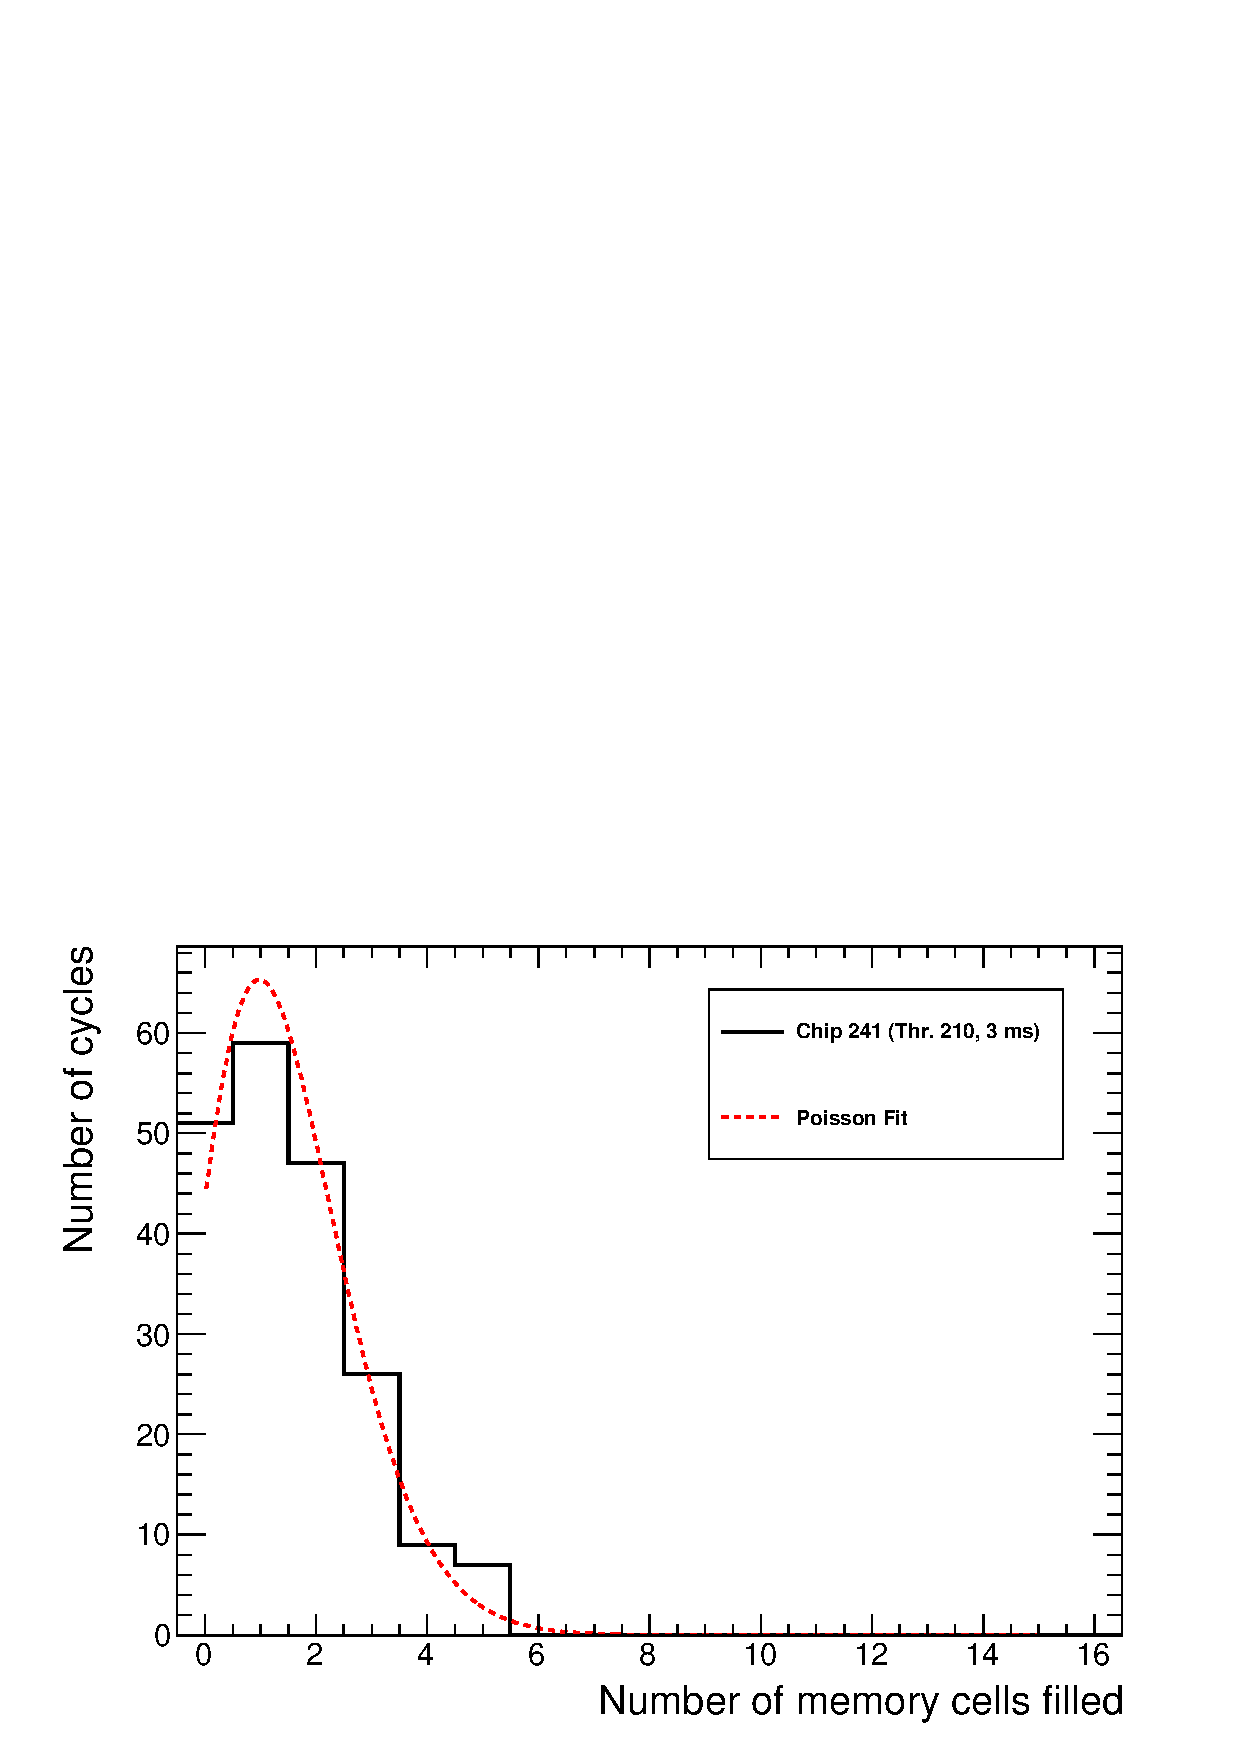
\includegraphics[width=1.\linewidth]{../Thesis_Plots/Commissioning/Plots/NumberMemFilled_Poisson.pdf}
    \caption{} \label{fig:MemPoison}
  \end{subfigure}
  \hfill
  \begin{subfigure}[t]{0.49\textwidth}
    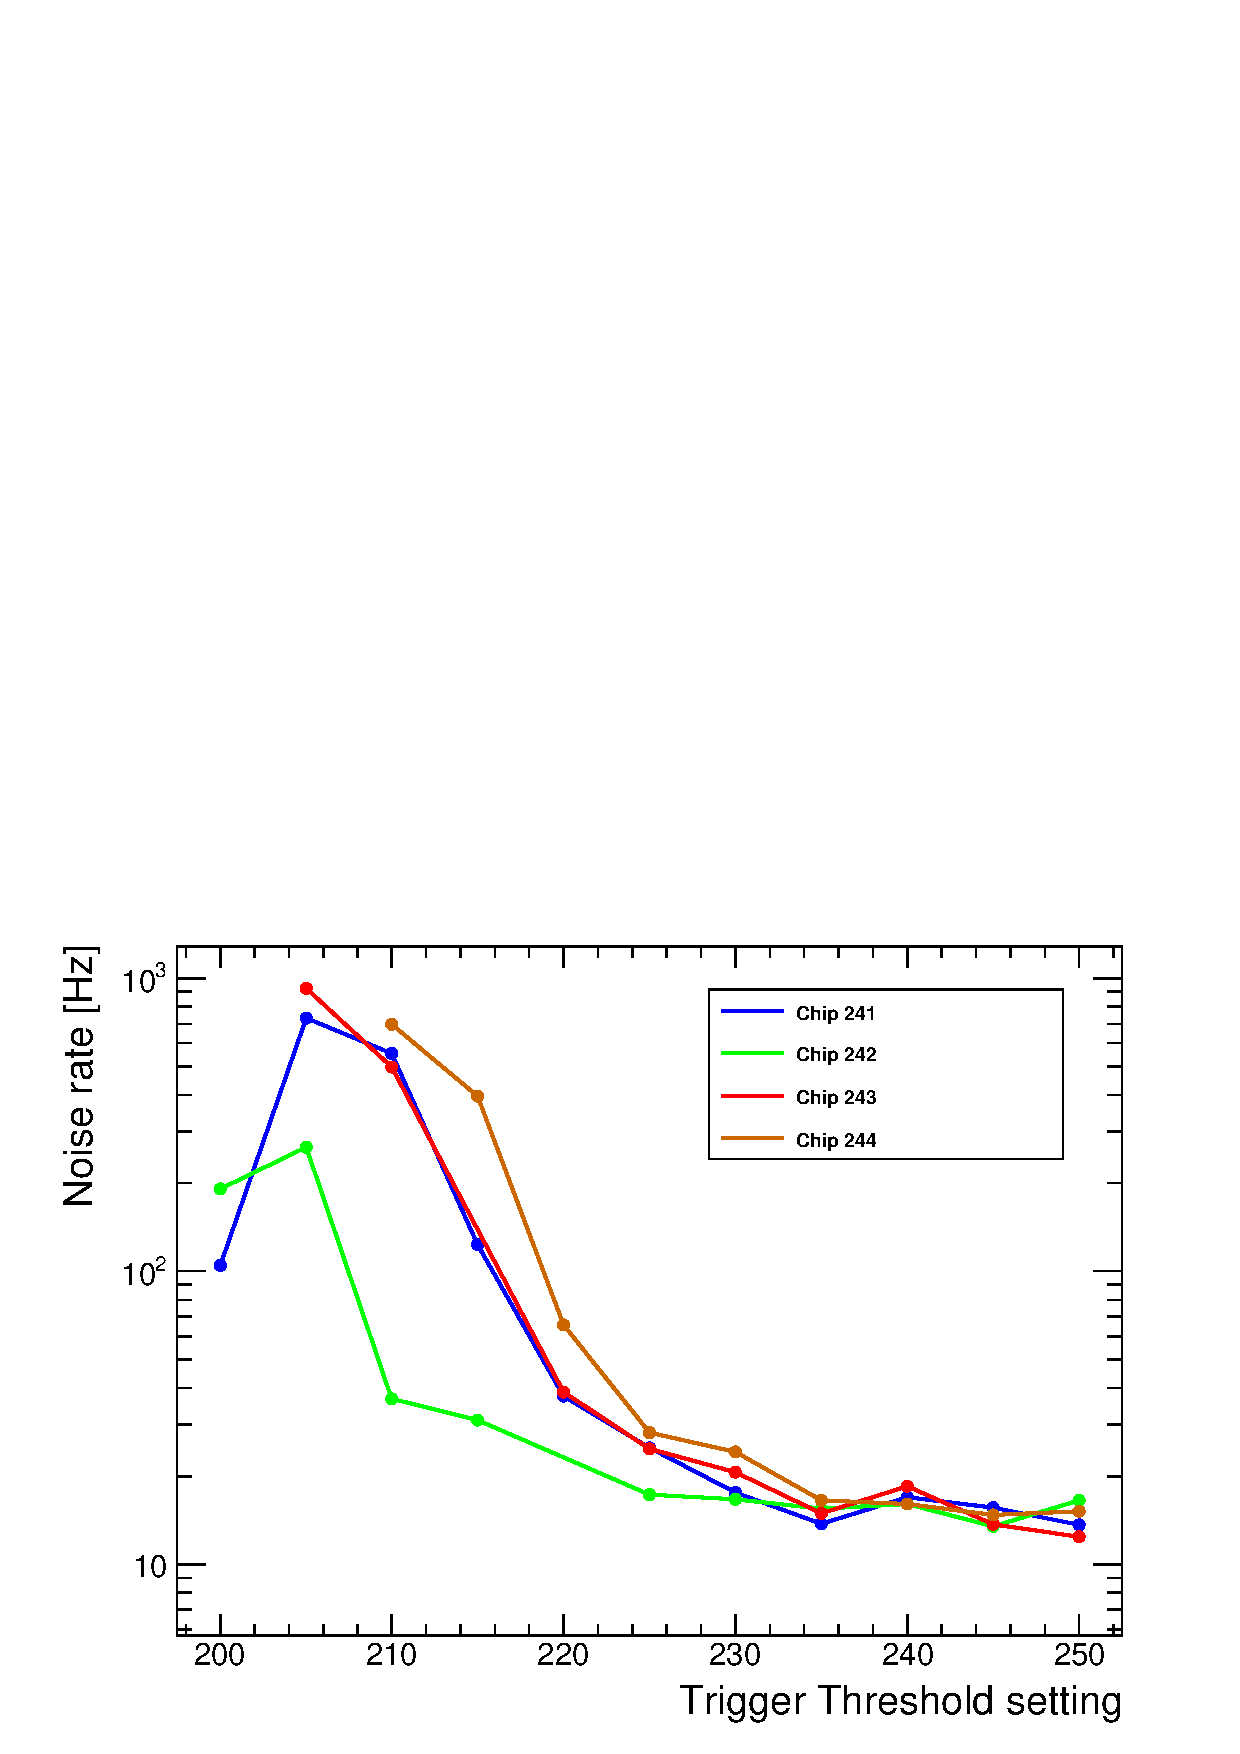
\includegraphics[width=1.\linewidth]{../Thesis_Plots/Commissioning/Plots/NoiseMeasurement_SM1.pdf}
    \caption{} \label{fig:DCRThr}
  \end{subfigure}
  \caption{\subref{fig:MemPoison}) Observed histogram of the number of memory cells filled per cycle for a typical chip with a trigger threshold of 210 and a time window $T$ of 3 ms. $\lambda_{mem}$ = 1.5 $\pm$ 0.1.\subref{fig:DCRThr}) Extracted noise rate as a function of the trigger threshold setting for a full board.}
\end{figure}

The figure \ref{fig:DCRThr} shows that noise decreases fast with increasing threshold until a plateau is reached. This plateau is the ideal area to set the threshold as noise is quite constant and does not vary a lot. In this figure, a threshold between 230 and 240 seems appropriate. As this method is complementary to the threshold scan, the region can be compared to where is the threshold put in terms of MIP value. For this board, a threshold of 230-240 corresponds to about a threshold 0.2-0.25 MIP which is well below 0.5 MIP and thus safe.

This method is very complementary to the threshold scan and can be used to set a relatively safe trigger threshold for all chips. It does not rely on a very precise measurement and has been shown to work well for all chips. Moreover, this method requires only minimal additional time to the commissioning procedure. A great understanding of the position of the trigger threshold relative to 0.5 MIP would greatly improve the characterization as well as the data taking efficiency of future AHCAL engineering prototypes.
